\chapter{Desarrollo del proyecto: Desarrollo del Algoritmo}

\section {Introducción}

Para poder desarrollar el algoritmo óptimo de toma de decisiones a la hora de apostar, es necesario también plantear “ante qué se quiere que reaccione el algoritmo”. Tal y como se ha comentado en el apartado anterior, hay dos modos de juego: uno contra el jugador y otro contra patrones predefinidos. Estos patrones,  son unos patrones fácilmente identificables a partir de cierto número de partidas jugadas, especialmente si se aplica el teorema de Bayes (ver apartado \ref{sec:bayes}).
Estos patrones genéricos, o predefinidos, son a los que se enfrentará el algoritmo óptimo en el caso de elegir el modo de juego de Máquina vs Máquina, eligiendo la opción de Algoritmo vs Patrón.
Cabe destacar que, tanto los algoritmos predefinidos como el algoritmo óptimo en verdad consiste en dos algoritmos (ya que el tratamiento de la información en la fase de Preflop es distinta a la del resto de fases posteriores), por lo que se tiene que considerar cada algoritmo para cada tipo de fase.

\section {Patrones predefinidos.}

Como se mencionó en el apartado \ref{sec:opti}, se ha programado un algoritmo con intención de que sea un algoritmo de juego óptimo, pero lo que se ha programado, por decirlo de alguna manera, ha sido la base de dicho algoritmo. Para convertirse en un algoritmo óptimo, el algoritmo tiene que “Entrenarse”, jugando contra otros algoritmos y contra jugadores. En este apartado, se va a tratar la parte del comportamiento de los algoritmos Predefinidos explicados previamente
Para ello, se van a crear 3 algoritmos predefinidos, basados en 3 de los patrones más comunes, como menciona Bill Chen en su libro\cite{chen}: Maniaco, Roca y Calling Station.
Estos tres patrones se van a desarrollar de la siguiente manera:
\begin{itemize}
\item Cada uno de los 3 patrones tendrá siempre una de las 3 acciones posibles como acción predominante:
\begin{itemize}
\item Maniaco: Subir
\item Roca: Pasar
\item Calling Station: Ver
\end{itemize}
\item Cada uno de los 3 patrones tendrá un comportamiento similar durante el preflop (únicamente con la fórmula de Chen como valor de referencia) como después del flop (con valor de jugada).
\item Cada uno de los 3 patrones tendrá una triple probabilidad para cada una de las jugadas de referencia posibles:
\begin{itemize}
\item Durante el preflop: si la mano pertenece a uno de los 8 grupos de Sklansky-Malmuth o si no pertenece a ninguno de ellos. Esto genera un total de 9 probabilidades triples de acción.
\item Después del preflop (también conocido como postflop): en función de cada una de las 10 posibles jugadas.
\end{itemize}
\end{itemize}

\subsection{Maniaco}

Para definir el comportamiento del patrón maniaco, se va a estimar el comportamiento agresivo de este patrón presentando siempre una gran probabilidad de subir comparado con las demás acciones posibles. 
Para estimarlo, se va a considerar que el comportamiento de este patrón será un comportamiento lineal.
En este caso, se van a definir los siguientes valores:
\begin{itemize}
\item Probabilidad en caso de mejor jugada: [p,v,s]=[0,0.05,0.95]
\item Decremento de s: -0.05 x escalón.
\item Incremento de p: +0.025 x escalón.
\item El valor de $v=1-(s+p)$ en este caso significa que v irá en incremento por escalón de +0.025 x escalón.
\end{itemize}
Una vez definido esto, se crean las tablas para cada una de las rondas

\subsubsection{Preflop}

\begin{longtable}[c]{|c|c|c|c|}
\hline
\rowcolor{lightgray}Grupo Sklansky - Malmuth & \%pasar & \%ver & \%subir \\
\hline
Grupo 1 & 0 & 0,05 & 0,95 \\
\hline
Grupo 2 & 0,025 & 0,075 & 0,9 \\
\hline
Grupo 3 & 0,05 & 0,1 & 0,85 \\
\hline
Grupo 4 & 0,075 & 0,125 & 0,8 \\
\hline
Grupo 5 & 0,1 & 0,15 & 0,75 \\
\hline
Grupo 6 & 0,125 & 0,175 & 0,7 \\
\hline
Grupo 7 & 0,15 & 0,2 & 0,65 \\
\hline
Grupo 8 & 0,175 & 0,225 & 0,6 \\
\hline
Sin Grupo & 0,2 & 0,25 & 0,55\\
\hline

\end{longtable}

\subsubsection{Postflop}

\begin{longtable}[c]{|c|c|c|c|}
\hline
\rowcolor{lightgray}Jugada & \%pasar & \%ver & \%subir \\
\hline
Escalera real & 0 & 0,05 & 0,95 \\
\hline
Escalera de Color & 0,025 & 0,075 & 0,9 \\
\hline
Poker & 0,05 & 0,1 & 0,85 \\
\hline
Full & 0,075 & 0,125 & 0,8 \\
\hline
Color & 0,1 & 0,15 & 0,75 \\
\hline
Escalera & 0,125 & 0,175 & 0,7 \\
\hline
Trio & 0,15 & 0,2 & 0,65 \\
\hline
Doble pareja & 0,175 & 0,225 & 0,6 \\
\hline
Pareja & 0,2 & 0,25 & 0,55\\
\hline
Carta Alta & 0,225 & 0,275 & 0,5\\
\hline
\end{longtable}

\subsection{Roca}

Este patrón es el más complicado de estimar de los tres patrones, ya que su comportamiento varía mucho en función de la fuerza de su jugada. Este comportamiento es muy difícil de estimar de una forma lineal, especialmente teniendo en cuenta que v tiene que aumentar y disminuir en función de la fuerza de la mano.
Por esto, se va a estimar el comportamiento de p y s como comportamientos parabólicos y, manteniendo v como $v=1-(p+s)$, también lo será. 
De esta manera, p tendrá su valor máximo en el peor de las jugadas, s tendrá su valor máximo en la mejor de las jugadas y v tendrá su valor más alto en punto donde p=s.
Con esto en cuenta, se ha creado el siguiente gráfico para mostrar de manera visual una forma aproximada de este comportamiento mostrado en la imagen \ref{fig:roca}.

\begin{figure}[h]
\centering
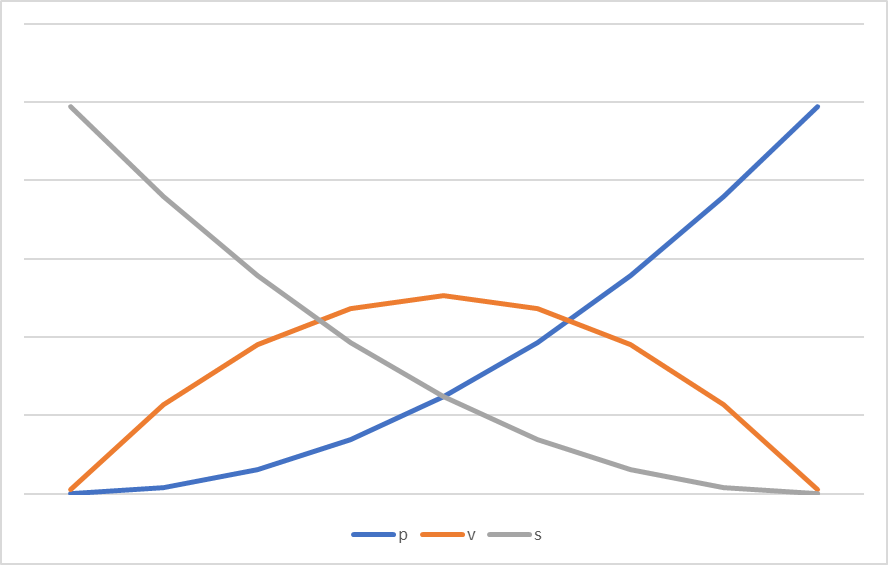
\includegraphics[width=0.45\textwidth]{figuras/roca.png}   
\caption{Relación entre s, v y p en el patrón roca\cite{propiaExcel}}
\label{fig:roca}
\end{figure}


\begin{itemize}
\item Probabilidad en caso de mejor jugada: [p,v,s]=[0,0.01,0.99] 
\item Probabilidad en caso de peor jugada: [p,v,s]=[0.99,0.01,0]
\end{itemize}

\subsubsection{Preflop}

En este caso, las parábolas de p y s son las siguientes:
\begin{itemize}
\item $p=0.01546875*esc^2 $
\item $s=0.01546875*(esc-8)^2$
\end{itemize}

Siendo esc $\in$[0,8], correspondiendo 0=Grupo 1 y 8=Sin grupo.

\begin{longtable}[c]{|c|c|c|c|}
\hline
\rowcolor{lightgray}Grupo Sklansky - Malmuth & \%pasar & \%ver & \%subir \\ \hline
Grupo 1 & 0 & 0,01 & 0,99 \\ \hline
Grupo 2 & 0,01546875 & 0,2265625 & 0,75796875 \\ \hline
Grupo 3 & 0,061875 & 0,38125 & 0,556875 \\ \hline
Grupo 4 & 0,13921875 & 0,4740625 & 0,38671875 \\ \hline
Grupo 5 & 0,2475 & 0,505 & 0,2475 \\ \hline
Grupo 6 & 0,38671875 & 0,4740625 & 0,13921875 \\ \hline
Grupo 7 & 0,556875 & 0,38125 & 0,061875 \\ \hline
Grupo 8 & 0,75796875 & 0,2265625 & 0,01546875 \\ \hline
Sin Grupo & 0,99 & 0,01 & 0 \\ \hline
\end{longtable}
\subsubsection{Postflop}

En este caso, las parábolas de p y s son las siguientes:
\begin{itemize}
\item $p=0.01222222*esc^2 $
\item $s=0.01222222*(esc-9)2$
\end{itemize}

Siendo esc $\in$[0,9], siendo cada uno de los escalones el valor entero de la jugada obtenida.

\begin{longtable}[c]{|c|c|c|c|}
\hline
\rowcolor{lightgray}Jugada & \%pasar & \%ver & \%subir \\ \hline
Escalera real & 0 & 0,01 & 0,99 \\ \hline
Escalera de Color & 0,01222222 & 0,20555556 & 0,78222222 \\ \hline
Pˇker & 0,04888889 & 0,35222222 & 0,59888889 \\ \hline
Full & 0,11 & 0,45 & 0,44 \\ \hline
Color & 0,19555556 & 0,49888889 & 0,30555556 \\ \hline
Escalera & 0,30555556 & 0,49888889 & 0,19555556 \\ \hline
Trio & 0,44 & 0,45 & 0,11 \\ \hline
Doble pareja & 0,59888889 & 0,35222222 & 0,04888889 \\ \hline
Pareja & 0,78222222 & 0,20555556 & 0,01222222 \\ \hline
Carta alta & 0,99 & 0,01 & 0 \\ \hline
\end{longtable}

\subsection{Calling Station}

El comportamiento de este patrón va a ser bastante similar al de maniaco, únicamente priorizando la probabilidad de ver la apuesta por encima de subir. También se tendrá un comportamiento lineal, aunque en este caso, la probabilidad que estará en función de las otras dos es la de pasar, ya que se le quiere dar más importancia a Ver.

En este caso, se van a definir los siguientes valores:
\begin{itemize}
\item Probabilidad en caso de mejor jugada: [p,v,s]=[0,0.85,0.15] 
\item Decremento de s: -0.0125 x escalón.
\item  Decremento de v: -0.025 x escalón.
\item El valor de p=1-(v+s) en este caso significa que p irá en incremento por escalón de +0.0375 x escalón.
\end{itemize}

\subsubsection{Preflop}
\begin{longtable}[c]{|c|c|c|c|}
\hline
\rowcolor{lightgray}Grupo Sklansky - Malmuth & \%pasar & \%ver & \%subir \\ \hline
Grupo 1 & 0 & 0,85 & 0,15 \\ \hline
Grupo 2 & 0,0375 & 0,825 & 0,1375 \\ \hline
Grupo 3 & 0,075 & 0,8 & 0,125 \\ \hline
Grupo 4 & 0,1125 & 0,775 & 0,1125 \\ \hline
Grupo 5 & 0,15 & 0,75 & 0,1 \\ \hline
Grupo 6 & 0,1875 & 0,725 & 0,0875 \\ \hline
Grupo 7 & 0,225 & 0,7 & 0,075 \\ \hline
Grupo 8 & 0,2625 & 0,675 & 0,0625 \\ \hline
Sin Grupo & 0,3 & 0,65 & 0,05 \\ \hline

\end{longtable}
\subsubsection{Postflop}

\begin{longtable}[c]{|c|c|c|c|}
\hline
\rowcolor{lightgray}Jugada & \%pasar & \%ver & \%subir \\ \hline
Escalera real & 0 & 0,85 & 0,15 \\ \hline
Escalera de Color & 0,0375 & 0,825 & 0,1375 \\ \hline
Pˇker & 0,075 & 0,8 & 0,125 \\ \hline
Full & 0,1125 & 0,775 & 0,1125 \\ \hline
Color & 0,15 & 0,75 & 0,1 \\ \hline
Escalera & 0,1875 & 0,725 & 0,0875 \\ \hline
Trio & 0,225 & 0,7 & 0,075 \\ \hline
Doble pareja & 0,2625 & 0,675 & 0,0625 \\ \hline
Pareja & 0,3 & 0,65 & 0,05 \\ \hline
Carta alta & 0,3375 & 0,625 & 0,0375 \\ \hline
\end{longtable}

\subsection{Cálculos para la formula de Bayes}
\label{sec:calcbayes}

En este apartado se va a desarrollar como se ha pasado de estos modelos a cifras para usar la fórmula de Bayes en el algoritmo óptimo.
Recordando el apartado \ref{sec:bayes}, son necesarios 4 datos para aplicar la fórmula:

\begin{itemize}
\item $p(A | B)$
\item  $p(A|\tilde{B})$
\item  $p(B)$
\item $p(\tilde{B})$
\end{itemize}

Teniendo en cuenta que A hace referencia al evento de \textit{ha tomado la acción} y B el evento de \textit{es un patrón concreto}, se puede reescribir de esta manera:
\begin{itemize}
\item $p(A | B)$: probabilidad de que, dado el patrón, haya tomado la acción
\item $ p(A|\tilde{B})$:  probabilidad de que, siendo un patron distinto al dado, haya tomado la acción
\item  $p(B)$: probabilidad de que sea ese patrón.
\item $p(tilde{B})$:probabilidad de queno  sea ese patrón.
\end{itemize}
La probabilidad de que sea o no sea el patrón irá variando en función de la toma de decisiones, puesto que será el resultado de la propia fórmula de Bayes (siendo el valor inicial 33\%). Por tanto, es necesario calcular $ p(A | B)$ y $p(A|\tilde{B})$.

Durante el preflop, ambos dependen del valor de la mano, se procede a analizar en qué casos ocurre cada acción. Hay que tener en cuenta que durante el preflop, las posibilidades son $\binom{52}{2}=1326$ posibles manos.


\begin{longtable}[c]{|c|c|c|c|}
\hline
\rowcolor{lightgray}Grupo Sklansky - Malmuth & Número de Manos del grupo & \% \\ \hline
Grupo 1 & 28 & 2,11\% \\ \hline
Grupo 2 & 30 & 2,26\% \\ \hline
Grupo 3 & 34 & 2,56\% \\ \hline
Grupo 4 & 46 & 3,47\% \\ \hline
Grupo 5 & 98 & 7,39\% \\ \hline
Grupo 6 & 108 & 8,14\% \\ \hline
Grupo 7 & 62 & 4,68\% \\ \hline
Grupo 8 & 154 & 11,61\% \\ \hline
Sin Grupo & 766 & 57,77\% \\ \hline
\end{longtable}

De esta manera, se ha realizado la suma ponderada con estos pesos a cada una de las acciones de los tres patrones durante el preflop, para determinar la probabilidad de que uno de esos patrones tome una acción.

\begin{longtable}[c]{|c|c|c|c|}
\hline
\rowcolor{lightgray}\multicolumn{4}{|c|}{p(A \textbar B) durante el preflop} \\ \hline
Patron & P(pasar) & P(ver) & P(subir) \\ \hline
Maniaco & 0,16489442 & 0,21489442 & 0,62021116 \\ \hline
Roca & 0,74252333 & 0,15740809 & 0,10006858 \\ \hline
Calling Station & 0,24734163 & 0,68510558 & 0,06755279 \\ \hline
\end{longtable}

El caso de las rondas posteriores al Preflop, el procedimiento es idéntico. En este caso, el número de jugadas posibles es $\binom{52}{5}=$2.598.960 combinaciones.

\begin{longtable}[c]{|c|c|c|c|}
\hline
\rowcolor{lightgray}Jugada & Combinaciones posibles & \% \\ \hline
Escalera real & 4 & 0,00\% \\ \hline
Escalera de Color & 36 & 0,00\% \\ \hline
Pˇker & 624 & 0,02\% \\ \hline
Full & 3744 & 0,14\% \\ \hline
Color & 5108 & 0,20\% \\ \hline
Escalera & 10200 & 0,39\% \\ \hline
Trio & 54912 & 2,11\% \\ \hline
Doble pareja & 123552 & 4,75\% \\ \hline
Pareja & 1098240 & 42,26\% \\ \hline
Carta alta & 1302540 & 50,12\% \\ \hline
\end{longtable}

Con estos pesos, se puede hacer la suma ponderada, tal y como se ha hecho en el caso anterior.

Haciendo esta suma ponderada de cada uno de los patrones, se tienen los siguientes valores de $p(A | B)$ en rondas posteriores a preflop.


\begin{longtable}[c]{|c|c|c|c|}
\hline
\rowcolor{lightgray}\multicolumn{4}{|c|}{p(A | B) después del preflop} \\ \hline
Patron & P(pasar) & P(ver) & P(subir) \\ \hline
Maniaco & 0,20957483 & 0,25957483 & 0,53085034 \\ \hline
Roca & 0,86622952 & 0,12179945 & 0,01197102 \\ \hline
Calling Station & 0,31436224 & 0,64042517 & 0,04521259 \\ \hline
\end{longtable}

Ya habiendo calculado los posibles valores de$ p(A | B)$, se pueden calcular los valores de$ p(A | \tilde{B})$.
Yendo a la definición de$ p(A | \tilde{B})$, se encuentra que es el caso en que sin ser el algoritmo, se haya tomado esa acción. En otras palabras, se puede definer $ p(A | \tilde{B})$como que cualquiera de los otros algoritmos haya tomado esa acción. Teniendo esto en consideración, y teniendo en cuenta que solo hay 3 patrones, se puede definir como:

\[ 
p(A | \tilde{B})= p(A | x \cup y) = p(A | x) \cup p(A | y) =  p(A | x) + p(A | y) 
\]

Siendo x e y los otros patrones distintos de B.
De esta manera, se tienen todos los valores para el cálculo del teorema de Bayes.

\section {Desarrollo del algoritmo óptimo.}
\label{sec:optimus}

Este algoritmo tiene como objetivo calcular las probabilidades de tener una mano más fuerte que la del oponente, una mano similar a la del oponente o una mano peor que la del oponente; y con esa probabilidad, tomar una de las tres posibles acciones: ver la apuesta, de subir la apuesta o de pasar la apuesta. Para ello, se deben de tener en consideración siempre las cartas de las que se tiene información:

\begin{itemize}
\item \textbf{Información común para todas las fases de la ronda}

Durante cada fase de la ronda, siempre se van a tener los siguientes datos:
\begin{itemize}
\item La mano conocida: dos cartas, cada una con un número y un palo, que son dos cartas conocidas.
\item La mano del otro jugador: dos cartas, al igual que la propia mano, pero en este caso son cartas que van a ser desconocidas siempre hasta el final de la ronda. 
\item Cada carta es única, es decir, una carta no puede aparecer dos veces
\end{itemize} 
Con estos 3 datos, se puede apreciar que se tiene una incógnita que se debe suponer de cara a calcular las probabilidades arriba mencionadas, pero el tercer dato (la unicidad de las cartas) nos permite suponer cada una de las posibles manos del oponente y, con eso, poder calcular las probabilidades.

\item\textbf{Tablas de probabilidades: tabla de pesos relativos y tabla de probabilidad de acción del oponente}

Para todo el funcionamiento del algoritmo se va a partir de dos tablas: una tabla que va a recoger la probabilidad relativa de que el oponente tenga una mano y una segunda tabla que recoja la probabilidad de cada mano del oponente de tomar una decisión u otra.
La tabla de pesos relativos recoge todas las posibles combinaciones de cartas y un valor numérico, al que se denomina Peso relativo (P$_r$), que puede tener valores entre 0 y 1. Este valor indica cómo de probable es que el oponente tenga una mano y otra y se irá actualizando con la decisión que tome el oponente.
La tabla de pesos relativos inicialmente tendrá estos valores.


\begin{longtable}[c]{|c|c|c|c|c|c|c|c|c|c|c|c|c|c|c|c|c|}
\hline
& 11 & 12 & 13 & 14 & 21 & 22 & 23 & 24 & 31 & 32 & 33 & 34 & 41 & 42 & 43 & 44 \\ \hline
1414 & 0 & 1 & 1 & 1 & 0 & 0 & 1 & 1 & 0 & 0 & 0 & 1 & 0 & 0 & 0 & 0 \\ \hline
1313 & 0 & 1 & 1 & 1 & 0 & 0 & 1 & 1 & 0 & 0 & 0 & 1 & 0 & 0 & 0 & 0 \\ \hline
1212 & 0 & 1 & 1 & 1 & 0 & 0 & 1 & 1 & 0 & 0 & 0 & 1 & 0 & 0 & 0 & 0 \\ \hline
1111 & 0 & 1 & 1 & 1 & 0 & 0 & 1 & 1 & 0 & 0 & 0 & 1 & 0 & 0 & 0 & 0 \\ \hline
1010 & 0 & 1 & 1 & 1 & 0 & 0 & 1 & 1 & 0 & 0 & 0 & 1 & 0 & 0 & 0 & 0 \\ \hline
909 & 0 & 1 & 1 & 1 & 0 & 0 & 1 & 1 & 0 & 0 & 0 & 1 & 0 & 0 & 0 & 0 \\ \hline
808 & 0 & 1 & 1 & 1 & 0 & 0 & 1 & 1 & 0 & 0 & 0 & 1 & 0 & 0 & 0 & 0 \\ \hline
707 & 0 & 1 & 1 & 1 & 0 & 0 & 1 & 1 & 0 & 0 & 0 & 1 & 0 & 0 & 0 & 0 \\ \hline
606 & 0 & 1 & 1 & 1 & 0 & 0 & 1 & 1 & 0 & 0 & 0 & 1 & 0 & 0 & 0 & 0 \\ \hline
505 & 0 & 1 & 1 & 1 & 0 & 0 & 1 & 1 & 0 & 0 & 0 & 1 & 0 & 0 & 0 & 0 \\ \hline
404 & 0 & 1 & 1 & 1 & 0 & 0 & 1 & 1 & 0 & 0 & 0 & 1 & 0 & 0 & 0 & 0 \\ \hline
303 & 0 & 1 & 1 & 1 & 0 & 0 & 1 & 1 & 0 & 0 & 0 & 1 & 0 & 0 & 0 & 0 \\ \hline
202 & 0 & 1 & 1 & 1 & 0 & 0 & 1 & 1 & 0 & 0 & 0 & 1 & 0 & 0 & 0 & 0 \\ \hline
1413 & 1 & 1 & 1 & 1 & 1 & 1 & 1 & 1 & 1 & 1 & 1 & 1 & 1 & 1 & 1 & 1 \\ \hline
1412 & 1 & 1 & 1 & 1 & 1 & 1 & 1 & 1 & 1 & 1 & 1 & 1 & 1 & 1 & 1 & 1 \\ \hline
1411 & 1 & 1 & 1 & 1 & 1 & 1 & 1 & 1 & 1 & 1 & 1 & 1 & 1 & 1 & 1 & 1 \\ \hline
1410 & 1 & 1 & 1 & 1 & 1 & 1 & 1 & 1 & 1 & 1 & 1 & 1 & 1 & 1 & 1 & 1 \\ \hline
1409 & 1 & 1 & 1 & 1 & 1 & 1 & 1 & 1 & 1 & 1 & 1 & 1 & 1 & 1 & 1 & 1 \\ \hline
1408 & 1 & 1 & 1 & 1 & 1 & 1 & 1 & 1 & 1 & 1 & 1 & 1 & 1 & 1 & 1 & 1 \\ \hline
1407 & 1 & 1 & 1 & 1 & 1 & 1 & 1 & 1 & 1 & 1 & 1 & 1 & 1 & 1 & 1 & 1 \\ \hline
1406 & 1 & 1 & 1 & 1 & 1 & 1 & 1 & 1 & 1 & 1 & 1 & 1 & 1 & 1 & 1 & 1 \\ \hline
1405 & 1 & 1 & 1 & 1 & 1 & 1 & 1 & 1 & 1 & 1 & 1 & 1 & 1 & 1 & 1 & 1 \\ \hline
1404 & 1 & 1 & 1 & 1 & 1 & 1 & 1 & 1 & 1 & 1 & 1 & 1 & 1 & 1 & 1 & 1 \\ \hline
1403 & 1 & 1 & 1 & 1 & 1 & 1 & 1 & 1 & 1 & 1 & 1 & 1 & 1 & 1 & 1 & 1 \\ \hline
1402 & 1 & 1 & 1 & 1 & 1 & 1 & 1 & 1 & 1 & 1 & 1 & 1 & 1 & 1 & 1 & 1 \\ \hline
1312 & 1 & 1 & 1 & 1 & 1 & 1 & 1 & 1 & 1 & 1 & 1 & 1 & 1 & 1 & 1 & 1 \\ \hline
1311 & 1 & 1 & 1 & 1 & 1 & 1 & 1 & 1 & 1 & 1 & 1 & 1 & 1 & 1 & 1 & 1 \\ \hline
1310 & 1 & 1 & 1 & 1 & 1 & 1 & 1 & 1 & 1 & 1 & 1 & 1 & 1 & 1 & 1 & 1 \\ \hline
1309 & 1 & 1 & 1 & 1 & 1 & 1 & 1 & 1 & 1 & 1 & 1 & 1 & 1 & 1 & 1 & 1 \\ \hline
1308 & 1 & 1 & 1 & 1 & 1 & 1 & 1 & 1 & 1 & 1 & 1 & 1 & 1 & 1 & 1 & 1 \\ \hline
1307 & 1 & 1 & 1 & 1 & 1 & 1 & 1 & 1 & 1 & 1 & 1 & 1 & 1 & 1 & 1 & 1 \\ \hline
1306 & 1 & 1 & 1 & 1 & 1 & 1 & 1 & 1 & 1 & 1 & 1 & 1 & 1 & 1 & 1 & 1 \\ \hline
1305 & 1 & 1 & 1 & 1 & 1 & 1 & 1 & 1 & 1 & 1 & 1 & 1 & 1 & 1 & 1 & 1 \\ \hline
1304 & 1 & 1 & 1 & 1 & 1 & 1 & 1 & 1 & 1 & 1 & 1 & 1 & 1 & 1 & 1 & 1 \\ \hline
1303 & 1 & 1 & 1 & 1 & 1 & 1 & 1 & 1 & 1 & 1 & 1 & 1 & 1 & 1 & 1 & 1 \\ \hline
1302 & 1 & 1 & 1 & 1 & 1 & 1 & 1 & 1 & 1 & 1 & 1 & 1 & 1 & 1 & 1 & 1 \\ \hline
1211 & 1 & 1 & 1 & 1 & 1 & 1 & 1 & 1 & 1 & 1 & 1 & 1 & 1 & 1 & 1 & 1 \\ \hline
1210 & 1 & 1 & 1 & 1 & 1 & 1 & 1 & 1 & 1 & 1 & 1 & 1 & 1 & 1 & 1 & 1 \\ \hline
1209 & 1 & 1 & 1 & 1 & 1 & 1 & 1 & 1 & 1 & 1 & 1 & 1 & 1 & 1 & 1 & 1 \\ \hline
1208 & 1 & 1 & 1 & 1 & 1 & 1 & 1 & 1 & 1 & 1 & 1 & 1 & 1 & 1 & 1 & 1 \\ \hline
1207 & 1 & 1 & 1 & 1 & 1 & 1 & 1 & 1 & 1 & 1 & 1 & 1 & 1 & 1 & 1 & 1 \\ \hline
1206 & 1 & 1 & 1 & 1 & 1 & 1 & 1 & 1 & 1 & 1 & 1 & 1 & 1 & 1 & 1 & 1 \\ \hline
1205 & 1 & 1 & 1 & 1 & 1 & 1 & 1 & 1 & 1 & 1 & 1 & 1 & 1 & 1 & 1 & 1 \\ \hline
1204 & 1 & 1 & 1 & 1 & 1 & 1 & 1 & 1 & 1 & 1 & 1 & 1 & 1 & 1 & 1 & 1 \\ \hline
1203 & 1 & 1 & 1 & 1 & 1 & 1 & 1 & 1 & 1 & 1 & 1 & 1 & 1 & 1 & 1 & 1 \\ \hline
1202 & 1 & 1 & 1 & 1 & 1 & 1 & 1 & 1 & 1 & 1 & 1 & 1 & 1 & 1 & 1 & 1 \\ \hline
1110 & 1 & 1 & 1 & 1 & 1 & 1 & 1 & 1 & 1 & 1 & 1 & 1 & 1 & 1 & 1 & 1 \\ \hline
1109 & 1 & 1 & 1 & 1 & 1 & 1 & 1 & 1 & 1 & 1 & 1 & 1 & 1 & 1 & 1 & 1 \\ \hline
1108 & 1 & 1 & 1 & 1 & 1 & 1 & 1 & 1 & 1 & 1 & 1 & 1 & 1 & 1 & 1 & 1 \\ \hline
1107 & 1 & 1 & 1 & 1 & 1 & 1 & 1 & 1 & 1 & 1 & 1 & 1 & 1 & 1 & 1 & 1 \\ \hline
1106 & 1 & 1 & 1 & 1 & 1 & 1 & 1 & 1 & 1 & 1 & 1 & 1 & 1 & 1 & 1 & 1 \\ \hline
1105 & 1 & 1 & 1 & 1 & 1 & 1 & 1 & 1 & 1 & 1 & 1 & 1 & 1 & 1 & 1 & 1 \\ \hline
1104 & 1 & 1 & 1 & 1 & 1 & 1 & 1 & 1 & 1 & 1 & 1 & 1 & 1 & 1 & 1 & 1 \\ \hline
1103 & 1 & 1 & 1 & 1 & 1 & 1 & 1 & 1 & 1 & 1 & 1 & 1 & 1 & 1 & 1 & 1 \\ \hline
1102 & 1 & 1 & 1 & 1 & 1 & 1 & 1 & 1 & 1 & 1 & 1 & 1 & 1 & 1 & 1 & 1 \\ \hline
1009 & 1 & 1 & 1 & 1 & 1 & 1 & 1 & 1 & 1 & 1 & 1 & 1 & 1 & 1 & 1 & 1 \\ \hline
1008 & 1 & 1 & 1 & 1 & 1 & 1 & 1 & 1 & 1 & 1 & 1 & 1 & 1 & 1 & 1 & 1 \\ \hline
1007 & 1 & 1 & 1 & 1 & 1 & 1 & 1 & 1 & 1 & 1 & 1 & 1 & 1 & 1 & 1 & 1 \\ \hline
1006 & 1 & 1 & 1 & 1 & 1 & 1 & 1 & 1 & 1 & 1 & 1 & 1 & 1 & 1 & 1 & 1 \\ \hline
1005 & 1 & 1 & 1 & 1 & 1 & 1 & 1 & 1 & 1 & 1 & 1 & 1 & 1 & 1 & 1 & 1 \\ \hline
1004 & 1 & 1 & 1 & 1 & 1 & 1 & 1 & 1 & 1 & 1 & 1 & 1 & 1 & 1 & 1 & 1 \\ \hline
1003 & 1 & 1 & 1 & 1 & 1 & 1 & 1 & 1 & 1 & 1 & 1 & 1 & 1 & 1 & 1 & 1 \\ \hline
1002 & 1 & 1 & 1 & 1 & 1 & 1 & 1 & 1 & 1 & 1 & 1 & 1 & 1 & 1 & 1 & 1 \\ \hline
908 & 1 & 1 & 1 & 1 & 1 & 1 & 1 & 1 & 1 & 1 & 1 & 1 & 1 & 1 & 1 & 1 \\ \hline
907 & 1 & 1 & 1 & 1 & 1 & 1 & 1 & 1 & 1 & 1 & 1 & 1 & 1 & 1 & 1 & 1 \\ \hline
906 & 1 & 1 & 1 & 1 & 1 & 1 & 1 & 1 & 1 & 1 & 1 & 1 & 1 & 1 & 1 & 1 \\ \hline
905 & 1 & 1 & 1 & 1 & 1 & 1 & 1 & 1 & 1 & 1 & 1 & 1 & 1 & 1 & 1 & 1 \\ \hline
904 & 1 & 1 & 1 & 1 & 1 & 1 & 1 & 1 & 1 & 1 & 1 & 1 & 1 & 1 & 1 & 1 \\ \hline
903 & 1 & 1 & 1 & 1 & 1 & 1 & 1 & 1 & 1 & 1 & 1 & 1 & 1 & 1 & 1 & 1 \\ \hline
902 & 1 & 1 & 1 & 1 & 1 & 1 & 1 & 1 & 1 & 1 & 1 & 1 & 1 & 1 & 1 & 1 \\ \hline
807 & 1 & 1 & 1 & 1 & 1 & 1 & 1 & 1 & 1 & 1 & 1 & 1 & 1 & 1 & 1 & 1 \\ \hline
806 & 1 & 1 & 1 & 1 & 1 & 1 & 1 & 1 & 1 & 1 & 1 & 1 & 1 & 1 & 1 & 1 \\ \hline
805 & 1 & 1 & 1 & 1 & 1 & 1 & 1 & 1 & 1 & 1 & 1 & 1 & 1 & 1 & 1 & 1 \\ \hline
804 & 1 & 1 & 1 & 1 & 1 & 1 & 1 & 1 & 1 & 1 & 1 & 1 & 1 & 1 & 1 & 1 \\ \hline
803 & 1 & 1 & 1 & 1 & 1 & 1 & 1 & 1 & 1 & 1 & 1 & 1 & 1 & 1 & 1 & 1 \\ \hline
802 & 1 & 1 & 1 & 1 & 1 & 1 & 1 & 1 & 1 & 1 & 1 & 1 & 1 & 1 & 1 & 1 \\ \hline
706 & 1 & 1 & 1 & 1 & 1 & 1 & 1 & 1 & 1 & 1 & 1 & 1 & 1 & 1 & 1 & 1 \\ \hline
705 & 1 & 1 & 1 & 1 & 1 & 1 & 1 & 1 & 1 & 1 & 1 & 1 & 1 & 1 & 1 & 1 \\ \hline
704 & 1 & 1 & 1 & 1 & 1 & 1 & 1 & 1 & 1 & 1 & 1 & 1 & 1 & 1 & 1 & 1 \\ \hline
703 & 1 & 1 & 1 & 1 & 1 & 1 & 1 & 1 & 1 & 1 & 1 & 1 & 1 & 1 & 1 & 1 \\ \hline
702 & 1 & 1 & 1 & 1 & 1 & 1 & 1 & 1 & 1 & 1 & 1 & 1 & 1 & 1 & 1 & 1 \\ \hline
605 & 1 & 1 & 1 & 1 & 1 & 1 & 1 & 1 & 1 & 1 & 1 & 1 & 1 & 1 & 1 & 1 \\ \hline
604 & 1 & 1 & 1 & 1 & 1 & 1 & 1 & 1 & 1 & 1 & 1 & 1 & 1 & 1 & 1 & 1 \\ \hline
603 & 1 & 1 & 1 & 1 & 1 & 1 & 1 & 1 & 1 & 1 & 1 & 1 & 1 & 1 & 1 & 1 \\ \hline
602 & 1 & 1 & 1 & 1 & 1 & 1 & 1 & 1 & 1 & 1 & 1 & 1 & 1 & 1 & 1 & 1 \\ \hline
504 & 1 & 1 & 1 & 1 & 1 & 1 & 1 & 1 & 1 & 1 & 1 & 1 & 1 & 1 & 1 & 1 \\ \hline
503 & 1 & 1 & 1 & 1 & 1 & 1 & 1 & 1 & 1 & 1 & 1 & 1 & 1 & 1 & 1 & 1 \\ \hline
502 & 1 & 1 & 1 & 1 & 1 & 1 & 1 & 1 & 1 & 1 & 1 & 1 & 1 & 1 & 1 & 1 \\ \hline
403 & 1 & 1 & 1 & 1 & 1 & 1 & 1 & 1 & 1 & 1 & 1 & 1 & 1 & 1 & 1 & 1 \\ \hline
402 & 1 & 1 & 1 & 1 & 1 & 1 & 1 & 1 & 1 & 1 & 1 & 1 & 1 & 1 & 1 & 1 \\ \hline
302 & 1 & 1 & 1 & 1 & 1 & 1 & 1 & 1 & 1 & 1 & 1 & 1 & 1 & 1 & 1 & 1 \\ \hline
\end{longtable}

Representando cada fila una combinación de dos cartas y cada columna el palo (T= tréboles, P= picas, D=Diamantes y C=Corazones) de cada una de las cartas. Por ejemplo, si se toma el valor de la fila 807 y la columna CD, ese Peso relativo corresponde a la probabilidad de que el oponente tenga un 8 de corazones y un 7 de diamantes en función de sus acciones a lo largo de la partida.
Como se puede observar, hay varias combinaciones que siempre tendrán una probabilidad de 0. Estas combinaciones ocurren únicamente en las parejas ya que:
\begin{itemize} 
\item Al ser las cartas únicas, no puede haber dos cartas iguales. Por tanto, una pareja de dos cartas del mismo palo (por ejemplo, tener dos 9 de diamantes) es imposible. Por tanto, estos casos siempre tendrán probabilidad de 0.
\item Al ser parejas, el orden de las cartas no influye. Es decir, tener un As de diamantes y un As de picas es lo mismo que tener un As de picas y un As de diamantes. Por esta razón, a las posibilidades repetidas, se les ha dado valor 0 para evitar valores duplicados.
\end{itemize} 
A pesar de ser combinaciones imposibles de conseguir, se ha decidido mantenerlas por comodidad, ya que al mantenerlas se puede crear una matriz con todas las posibilidades. En caso de eliminarlas, habría que hacer dos matrices para recoger esos datos: una para las parejas y otra para las combinaciones de cartas que no sean parejas, dificultando el cálculo matemático.
También cada vez que una carta sea conocida, todas las combinaciones posibles con esa carta se convertirán en 0.
Para actualizar estos valores a lo largo de la partida, se tiene la segunda tabla, la denominada tabla de probabilidad triple de acción del oponente, o simplemente tabla de probabilidad triple de acción. Por cada jugador distinto del algoritmo, sería necesaria una tabla independiente, pero ya que solo hay únicamente dos jugadores, esto se simplifica a una única tabla.
Antes de hablar de la tabla, se va a explicar el concepto de probabilidad triple de acción del oponente. La probabilidad triple de acción del oponente es un conjunto de tres valores entre 0 y 1 {p, v, s} que representan cómo de probable es que el adversario tome una de las tres posibles acciones (pasar (p), ver (v) y subir (s)) desde el punto de vista del algoritmo. En otras palabras, es un conjunto de tres números que representa la probabilidad de que ocurra el evento de pasar la apuesta, el evento de ver la apuesta o el evento de subir la apuesta para cada mano.
Como estoy hablando de probabilidades, y sabiendo que siempre que ocurrir uno de los tres eventos, se cumple que $ p+v+s=1$.
La tabla de probabilidad triple de acción recoge la probabilidad triple de acción para cada combinación de cartas del oponente. Estas probabilidades serán
La tabla tendrá un aspecto como este para cada combinación de cartas:


\begin{longtable}[c]{|c|c|c|c|}
\hline
 & \%Pasar & \%Ver & \%Subir \\ \hline
$N_1P_1N_2P_2$ & p & v & S \\ \hline
\end{longtable}

Siendo $ N_1$ y $P_1$el número y palo de la primera carta y $N_2$ y $P_2$ el número y palo de la segunda

Dado que estos valores son probabilidades de acción, estos valores cambiarán con el paso de las rondas.
Previamente se ha mencionado que los valores de la tabla de pesos relativos se actualizarían con las acciones del oponente y los valores de la tabla de probabilidad de acción del oponente. En función de la acción del oponente, se multiplica el valor de la tabla de la tabla de pesos relativos para esa combinación por el valor de la acción elegida de la tabla de probabilidad de acción del oponente que tenga esa mano.
Se pone un ejemplo:
Si se tiene los siguientes pesos en la tabla de pesos relativos:
\[
P_r \{10\clubsuit 7\spadesuit\} = 0,7
\]
\[
P_r\{\textcolor{red}{09\vardiamondsuit 03\varheartsuit}\} = 0,3
\]
\[
P_r \{\textcolor{red}{A\vardiamondsuit} Q\spadesuit\} = 0,64
\]
Y las siguientes probabilidades triples de acción:
\[
PtA \{10\clubsuit 7\spadesuit\} = \{0,24; 0,61; 0,15\}
\]
\[
PtA \{\textcolor{red}{09\vardiamondsuit 03\varheartsuit}\} = \{0,61; 0,3; 0,09\}
\]
\[
PtA \{\textcolor{red}{A\vardiamondsuit} Q\spadesuit\} = \{0,03; 0,28; 0,69\}
\]
Si el oponente ve la apuesta, los nuevos valores de los pesos en la tabla serían:
\[
P_r \{10\clubsuit 7\spadesuit\}  = 0,7*0,61=0,427
\]
\[
P_r\{\textcolor{red}{09\vardiamondsuit 03\varheartsuit}\} = 0,3*0,3 = 0,09
\]
\[
P_r \{\textcolor{red}{A\vardiamondsuit} Q\spadesuit\} = 0,64*0,28 = 0,1792
\]
Como se puede observar, en caso de ver la apuesta, la combinación más probable de las tres consideradas sería $\{10\clubsuit 7\spadesuit\}$ y la menos probable sería $\{\textcolor{red}{09\vardiamondsuit 03\varheartsuit}\}$. También se aprecia que la probabilidad de que sea  $\{\textcolor{red}{A\vardiamondsuit} Q\spadesuit\}$ también ha bajado, pues con esa mano lo más probable hubiera sido subir la apuesta.
Una vez explicado estas bases, se pasa a explicar el funcionamiento del algoritmo.
Para empezar, se tiene considerar que la información conocida en las fases varía:
\begin{itemize}
\item Durante el preflop, únicamente se tiene la mano 
\item Durante el flop se tiene la propia mano y 3 cartas comunes
\item Durante el turn, se tiene la propia mano y 4 cartas comunes
\item Durante el river, se tiene la propia mano y las 5 cartas comunes.
\end{itemize}
Por tanto, el comportamiento del algoritmo  se tiene que adaptar para que pueda reflejar esta variación de información.
Para ello, se procede a dividir el algoritmo en tres “partes”, cada una con un funcionamiento particular:
\begin{enumerate}
\item Cuando no se tiene información de las cartas de la mesa. (Preflop)
\item Cuando hay información de cartas de la mesa y aún quedan cartas por salir (Flop y Turn)
\item Cuando ya está toda la información de las cartas de la mesa (River)
\end{enumerate}

\end{itemize} 

El funcionamiento general de la actualización es calcular los factores de la mano propia, calcular la probabilidad triple de acción del algoritmo actualizar la tabla de triple probabilidad y, por ultimo,  actualizar la tabla de pesos del oponente con la acción tomada por el oponente y la tabla de triple probabilidad de acción del oponente. 

\subsection{Preflop}

En esta fase, solo se dispone de 2 cartas de información conocida, por lo tanto restan 50 cartas posibles, de las cuales cualquier combinación de esas 2 cartas podrían ser las que quedan en la mano del oponente, lo que significa un total de $\binom{50}{2} = 1225 $combinaciones posibles.
Otra de las peculiaridades de esta fase es que, puede que no haya habido ningún tipo de apuesta por parte del oponente al comienzo de esta apuesta, por lo que los pesos podrían ser iguales uno a otro.
Como ya se ha comentado en el apartado \ref{sec:chen} hablado previamente, la fuerza de una mano en el preflop se ha determinado mediante la fórmula de Chen. Es cierto que esta fórmula tiene sus limitaciones, pero como un indicador base nos sirve de guía de cara a automatizar este proceso.
Tal y como se mencionó en el apartado \ref{sec:chen}, Chen, según su experiencia, nos indicaba varias puntuaciones por las que se podría empezar a jugar una mano.\cite{krieger} Pero, en una partida de dos jugadores, no hay posiciones, ya que no hay jugadores intermedios entre un jugador y el Dealer. Pero partiendo de ese criterio, y del cruce con Sklansky-Malmuth (ver figura \ref{fig:sklansky},  se puede determinar qué manos ver, qué manos subir y qué manos desechar. 
Una de las cualidades que se busca  en el algoritmo es que sea imprevisible, por lo que se van a añadir porcentajes de acción, para que, aunque se tenga una acción predominante, no siempre sea preciso.
En función del valor de la fórmula de Chen, se establece esta valoración de triples probabilidades:


\begin{longtable}[c]{|c|c|c|c|}
\hline
\rowcolor{lightgray}Puntuación Chen & \%pasar & \%ver & \%subir \\ \hline
12-20 & 0 & 0,1 & 0,9 \\ \hline
10-11 & 0 & 0,25 & 0,75 \\ \hline
5*-9 & 0,25 & 0,65 & 0,1 \\ \hline
3,5-5** & 0,69 & 0,3 & 0,01 \\ \hline
Menor de 3,5 & 0,99 & 0,01 & 0 \\ \hline
\end{longtable}

Para esta valoraciones y asignar estos pesos,se han tomado en consideración los siguientes aspectos:
\begin{itemize}
\item Los pertenecientes al Grupo uno de Sklansky-Malmuth (12-20) son manos con las que son convenientes tomar la estrategia de subir la mano, por tanto, son manos que siempre se van a jugar. Además, son manos que, ante una subida, también son partidarias de resubir dicha subida.
\item Los pertenecientes al Grupo 2 (10-11) son manos con las que son convenientes tomar una estrategia agresiva pero no tanto como las del grupo anterior, por tanto, son manos que prácticamente siempre se van a jugar. Además, son manos que, ante una subida, también son partidarias de ver dicha subida, pero no de subirlas
\item Las manos pertenecientes a los grupos 3 al 6 (5*-9) son las manos que, según Chen, son manos jugables según la posición que se tenga. Por tanto, se puede asumir que son manos que suelen ver las apuestas, aunque ante resubidas, suelen pasar.  *Las manos de valor 5 incluidas aquí son únicamente las parejas (si bien la pareja de 5 es la única combinación de valor 5 según la fórmula de Chen que pertenece al grupo 6, considero que, dado que las otras parejas se pueden incluir aquí ya que son una jugada hecha y, además, al solo haber un oponente, no son tan fácil de superar como si hubiera más jugadores puesto que, a más jugadores, más posibilidades de que se forme una pareja con cualquiera de las cartas comunes.
\item Las manos pertenecientes a los grupos 7 y 8 (3,5-5**) son manos que son difíciles de ganar, pero aún se consideran con posibilidades según la clasificación de Sklansky-Malmuth. Tanto Chen como Krieger\cite{krieger} recomiendan que estas manos sean descartadas, por eso se le da un mayor peso a pasar que a ver. **Aquí no están incluidas las incluidas en el punto anterior, pero si están incluidas las combinaciones de AX de distinto palos siendo $X>9$ puesto que, aunque la fórmula de Chen les dé una valoración de 5, Malmuth-Sklansky las descarta como manos jugables. Se ha decidido incluirlas por un razonamiento similar al anterior punto: al haber un solo oponente esta combinación de cartas gana fuerza.
\item Manos por debajo de 3,5: son las combinaciones que están fuera de los grupos Sklansky-Malmuth, con la excepción mencionada en el punto anterior, por lo que son manos con muchas dificultades para ganar la jugada. Por ende, son manos prácticamente descartables.
\end{itemize}

De estos razonamientos se puede establecer una segunda tabla de probabilidad triple, ante la resubida en caso de que el oponente suba:

\begin{longtable}[c]{|c|c|c|c|}
\hline
\rowcolor{lightgray}Puntuación Chen & \%pasar & \%ver & \%subir \\ \hline
12-20 & 0 & 0,2 & 0,8 \\ \hline
10-11 & 0 & 0,8 & 0,2 \\ \hline
5*-9 & 0,85 & 0,1 & 0,05 \\ \hline
5 o menor & 0,99 & 0,01 & 0 \\ \hline
\end{longtable}


A medida que va avanzando la partida, se puede observar que se van perfilando las manos del oponente según sus acciones. 
Una vez obtenida la probabilidad de acción triple del algoritmo, es necesario ajustarla en función del algoritmo al que se enfrente. Para eso, se crea la función \textit{ajusteBayes}. Esta función calculará cual de los 3 patrones es el mas probable que sea y en función de a cual de los 3 sea el más probable según bayes (aplicando la fórmula del teorema de bayes a cada uno de los tres patrones), se ajustará la probabilidad para compensar la fortaleza de dicho patrón. En caso de que no se sepa identificar el patrón por cercanía de los patrones más probables mantendrá las probabilidades igual.

Independientemente de si no es capaz de identificar el patrón o no, almacenará estas tres probabilidades (la probabilidad de el oponente sea maniaco, sea Roca o sea Calling Station), almacenará los valores en un fichero para su reutilización en posteriores llamadas a la función.
\begin{verbatim}

ajusteBayes(triple, accion, ronda)
      [Maniaco,Roca, Calling Station] <- cargadeProbabilidades(ronda)
      PatronMasProbable<-comparaProbabilidades
      triple_actualizado<-ajuste(PatronMasProbable,accion,triple)
      return(triple_actualizado)
\end{verbatim}

El ajuste en cada ronda será en función del valor de la jugada y del patrón al que se enfrente, ya que cada uno de los patrones tienen debilidades, por lo que se modificarán los pesos en función de esas debilidades. 
Tras eso, es necesario actualizar la Tabla de Probabilidad de acción del oponente.
Para ello, se va a aplicar las tablas de probabilidades de acción de cada ronda para el algoritmo supuesto, creando la función \textit{CalculoProbabilidadAccion}.

\begin{verbatim}
CalculoProbabilidadAccion(mesa,mazo,tabla_triple,ronda)
      [Maniaco,Roca, Calling Station] <- cargadeProbabilidades(ronda)
      PatronMasProbable<-comparaProbabilidades
      valoresNuevosPatron <-cargadeValoresPatrones(ronda, Patron)
      para  cada  (ManoOp)
            {
            categoria<-ValorarJugada(ronda,ManoOp,mesa)
            tabla_triple[i]<-valoresNuevos[categoria]
            }
      return(tabla_triple)
\end{verbatim}

Dado que en esta ronda no hay cartas en Mesa, ese valor es 0.
Una vez actualizados los valores de acción y las tablas correspondientes, se continúa con la siguiente ronda de juego.

\subsection{Flop y Turn}
\label{sec:flopturn}

Se han agrupado ambas fases en este punto porque tienen una composición parecida: hay varias cartas comunes, pero aún quedan cartas por salir. Además, al haber al menos 5 cartas entre la mano y la mesa, la fórmula de Chen deja de ser efectiva pues ya hay jugadas. Ahora las jugadas siguen la puntuación mencionada previamente (0 a 9, siendo 0 carta más alta y 9 Escalera Real).

Lo primero que hay que hacer es actualizar la tabla de probabilidades con las cartas reveladas en la fase correspondiente (3 cartas en Flop y 1 en Turn), haciendo que todas las combinaciones de cartas que incluyan dichas cartas tengan probabilidad 0.

Despues, se puede empezar a valorar la situación con la información que se tiene.
En este caso, no se puede hacer un simple cálculo para determinar qué puede tener el oponente, puesto que hay muchas más variables posibles en lo que se refiere a las posibles combinaciones de mano.
Para poder automatizar esto, se va a tomar como base las ideas plasmadas en Algorithms and Assessment in Computer Póker , la tesis doctoral de Darse Billings de la universidad de Alberta\cite{doctor}. En la tesis, habla de distintas estrategias para cómo automatizar el juego de póker.
En dicha tesis, se define el valor de Fuerza de Mano (FM), que es la probabilidad de que una mano sea mejor que la del oponente, al igual que el Valor Potencial de la Mano (VPM), que es la fuerza potencial con las posteriores cartas.
Estas definiciones sirven de base para este proyecto, aunque se van a realizar modificaciones sobre eso para que se amolden a este algoritmo. Para empezar, se va a calcular cómo de buena es la mano con respecto a las posibles manos del oponente. Pero antes de eso, es necesario hacer una simplificación, de cara a ayudar a los cálculos: únicamente se van a tomar en consideración variaciones en la puntuación directa de la jugada, no en su desempate. Es decir, si cada jugador tiene una pareja, se van a considerar como “jugadas iguales”, aunque en la práctica esto no tenga que ser estrictamente cierto.
Con esto, se puede empezar a ver cómo de buena es esta mano, para eso se comprueba si, con cada combinación de dos cartas posibles del oponente su jugada es mejor, peor o igual que la del jugador.
\begin{verbatim}
CalcularFuerzaMano(valorjugadaJugador, Mesa)
      *Considerando cada una de las posibles manos del oponente*
      para cada (ManoOp):
            {
            valorjugadaOp <- calcularValorJugada(ManoO,Mesa);
            si valorjugadaOp > valorjugadaJugador 
                  ValorSuperior= ValorSuperior +1* P{ManoOp};
            si valorjugadaOp== valorjugadaJugador 
                   ValorIgual= ValorIgual +1* P{ManoOp};
            si valorjugadaOp < valorjugadaJugador -
                  ValorInferior= ValorInferior +1* P{ManoOp};	
            }
      FMsuperior=(ValorSuperior)/(TotalValores)
      FMigual=(ValorIgual)/( TotalValores)
      FMinferior=(ValorInferior)/( TotalValores)
\end{verbatim}
Siendo FMsuperior el porcentaje en que la mano es superior a la del oponente, FMigual el porcentaje en que la mano es igual a la del oponente,FMinferior el porcentaje en que la mano es inferior a la del oponente y P$\{ManoOponente\}$ al valor P$_r$ de dicha mano.
El hecho de tener los valores de P$_r$ como parte de los cálculos implica que la fuerza de la mano del algoritmo varía según su propia estimación de las manos que haga del oponente (ya que, hay 10 ManoOponente que hagan una mejor jugada que la del algoritmo pero tienen un P$_r$ de 0.1 cada una la mano es más fuerte que si tienen un P$_r$ de 0.6 y viceversa).

En estas fases, este valor FM no es suficiente para perfilar una estrategia, pues aún quedan cartas por salir e información que revelarse: en el Flop 2 cartas y en el Turn 1 carta.
Para esto, hay que intentar suponer cómo evolucionarán las manos con las posibles cartas. Hay dos maneras de enfocarlo:

\begin{enumerate}
\item Durante el flop considerar ambas posibles cartas 
\item Considerar únicamente la siguiente carta a salir
\end{enumerate}

En el primer caso, se tendría que considerar, para cada una de las 1081 posibles manos del oponente, cada una de las posibles 45 cartas restantes del mazo y, así mismo, para cada una de esas 45 cartas restantes, cómo afectaría la jugada para cada una de las 44 cartas restantes durante el flop y luego durante el turn considerar de nuevo las 44 cartas restantes para cada mano posible del oponente, aunque solo habría que calcularlo una vez. 
Mientras que, en el segundo caso, únicamente se tiene que considerar para cada una de las posibles manos del oponente, cómo afectaría a la jugada la aparición de cada una de las posibles 45 cartas restantes del mazo durante el flop y para el turn considerar para cada una de las 1035 manos posibles del oponente la variación de la jugada con las 44 cartas restantes del mazo. Es decir, hacer dos cálculos uno para cada fase.


Se va a utilizar la segunda opción, por sencillez de computación y rendimiento a la hora de tiempos de ejecución. Si bien es cierto que se pierde precisión a la hora de estimar, se gana bastante en rendimiento ya que son menos combinaciones a tener en cuenta.

Para ello, se calcula el Valor Potencial de la Mano (VPM), de manera similar a cómo lo calcula Darse Billings en su tesis. Es decir, para cada mano del oponente, se analiza si se parte de estar en ventaja, en igualdad o en inferioridad y se estudia cómo esa situación mejora, empeora o se queda igual (dando lugar a un total de 9 posibilidades)

\begin{verbatim}
CalcularPotencial(valorjugadaJugador, Mesa)
      *Considerando cada una de las posibles manos del oponente*
      para cada (ManoOp):
            {
            valorjugadaOponente <- calcularValorJugada(ManoOp,Mesa);
            si valorjugadaOponente > valorjugadaJugador 
                  ValorSuperior= ValorSuperior +1* P{ManoOp};
                  previo=1
            si valorjugadaOponente == valorjugadaJugador 
                  ValorIgual= ValorIgual +1* P{ManoOp};
                  previo=2
            si valorjugadaOponente < valorjugadaJugador -
                  ValorInferior= ValorInferior +1* P{ManoOp};	
                  previo=3
            *Considerando cada una de las posibles cartasrestantes*
            para cada (CartaRestamte)
                  {
                  Mesa'= Mesa + Carta Restante
                  valorjugadaOponente'<-calcularValorJugada(ManoOp,Mesa');
                  valorjugadaJugador'<-calcularValorJugada(Mano,Mesa');
                  si valorjugadaOponente' > valorjugadaJugador '
                        Pierde[fila]= Pierde[fila] +1* P{ManoOp};
                  si valorjugadaOponente' == valorjugadaJugador '
                        Empata[fila]= Empata +1* P{ManoOp};
                  si valorjugadaOponente' < valorjugadaJugador'
                        Gana[fila]= Gana +1* P{ManoOp};	
                  }
            }
      PotPositivo = Gana/ValorSuperior;
      PotNegativo = Pierde/ValorInferior;
\end{verbatim}

Siendo el  PotPositivo cómo puede mejorar una mano (es decir, de ir perdiendo a ganar una mano) y PotNegativo cómo puede empeorar la mano (es decir, de ir ganando a perder una mano)

Ahora que se tiene tanto FM como la posible variación con la siguiente carta se podría establecer ya una estrategia, pero hay más factores a tener en cuenta con respecto a esto.

Uno de estos factores son las cuotas, tambien llamadas \textit{odds}.

Lo primero, se van a calcular el \textit{odd} de mano, cuántas de las posibles cartas restantes mejoran la jugada. Para ello, se van a valorar cada una de las cartas que se desconocen. 

\begin{verbatim}
calculoOddMano(mano,mesa,mazo)
      para cada (ManoOponente):
            {
            valorjugadaJugador' <-calcularValorJugada(Mano,Mesa')
            si(valorjugadaJugador<valorjugadaJugador')
                  mejora++
            }
      OddMano=mejora/cartasMazo
\end{verbatim}

Después, se a calcular el \textit{odd} del bote, es decir, cual es la relación entre cuánto dinero hay en el bote y cuanto es necesario apostar. En otras palabras, el inverso de cuántas veces mas grande es el total de la apuesta con respecto a la cantidad a apostar.

\begin{verbatim}
calculoOddMano(ApuestaActualJugador, ApuestaActualOponente)
      Diff = ApuestaActualOponente-ApuestaActualJugador
      Bote = ApuestaActualJugador+ApuestaActualOponente+Diff
      OddBote=Diferencia/Bote
\end{verbatim}

Con estos factores, ya se tienen datos suficientes para calcular una probabilidad triple de acción para el algoritmo.
Teniendo en cuenta que p+v+s=1, la fórma más sencilla de conseguir que se cumpla esto siempre es que uno de los tres valores sea una combinación lineal de los otros dos. Debido a que la opción que se considera como “pasiva” es la opción de Ver, se va a reformular esa ecuación como v=1-(p+s). Es decir, que v será siempre una función de s y p
.
Teniendo todos los valores, se puede establecer una fórmula de cálculo genérico tanto para p como para s:
\[
X=FM + POT + Odds
\]


Dado se considera que no todos los factores tienen el mismo peso a la hora de tomar una decisión, la fórmula va a llevar pesos para garantizar que eso se cumple. 
Dado que la fuerza de la mano y el potencial de la mano son complementarios (ya que el Potencial de la mano utiliza un código similar al de la fuerza de Mano) van a tener una relación directa en la fórmula y compartir el mismo peso. Así mismo, tanto la fuerza de la mano como el potencial de esta deben tener un mayor peso en la fórmula para determinar si la apuesta es o no adecuada ya que, aunque el Odd sea muy favorable, debe tener menos peso a una mano que es dificil que mejore.. Para esto, se van a asignar un 80\% del peso a Fuerza y potencial, y el 20\% restante a los Odds.

De esta manera, se pueden sacar las probabilidades de Subir y de pasar una apuesta, y, por ende, de ver la mano.
\[
s= 0.8*(FMsuperior+(1- FMsuperior)*PotPositivo)+0.1*OddMano+0.1*OddBote
\]
\[
p=0.8*(FMinferior+(1-FMinferior)*PotNegativo)+0.1*(1-OddMano)+0.1*Oddbote
\]
\[
v=1-(p+s)
\]

Si bien ninguno de los 6 valores utilizados en p y s pueden ser mayor a 1 ni inferior a 0, es posible que en algunas situaciones s+p sean mayor a uno (por ejemplo, tener una pareja baja en la mano, hay muchas cartas que la mejoran, al igual que hay muchas que la empeoran). En el caso de que eso ocurra, la probabilidad de ver sería negativa, algo impensable. Por ello, es necesario hacer un ajuste proporcional para impedir que esto ocurra.

\[
s_i= 0.8*(FMsuperior+(1- FMsuperior)*PotPositivo)+0.1*OddMano+0.1*OddBote
\]
\[
p_i=0.8*(FMinferior+(1- FMinferior)*PotNegativo)+0.1*(1-OddMano)+0.1*Oddbote
\]
\[
v_i=|p_i+s_i-1|
\]
\[
t=s_i+v_i+p_i
\]

\[
s=\frac{s_ini}{t}  \quad  v=\frac{v_ini}{t} \quad  p=\frac{p_ini}{t}
\]

Después de eso, el paso final es la corrección de estos valores en función del patrón al que se enfrente el algoritmo. Para ello, se utilizará la función \textit{ajusteBayes}, mencionada en el apartado anterior. 

Antes se ha mencionado un factor que se ha mencionado que influenciaba en estas probabilidades, pero no se ha tomado en cuenta para la fórmula y es el factor de farol. Como se mencionó previamente, los faroles son una estrategia para apostar sin tener una mano ganadora, ya sea cuando no se tiene posibilidad de ganar una mano (farol puro) o cuando no se sabe si la mano puede llegar a ser una mano ganadora (semi farol).
Para representar este factor, así como para mantener la imprevisibilidad del algoritmo, se va a programar este comportamiento mediante un número aleatorio. Dado que son manos donde las probabilidades están en contra, el algoritmo solo va a considerar la posibilidad de \textit{echarse} un farol cuando p sea la mayor de las tres probabilidades, pero no siempre que vaya perdiendo será partidario de seguir esta estrategia, pues de hacer faroles constantemente acaba perdiendo fuerza. 

Por eso se determinará este comportamiento determinando si se hace el farol con un numero aleatorio entre 0 y 100, y si se cumple que  es mayor o igual a p, entonces se hará el farol.
En este caso, $v'=v+p/2$, $s'=s+p/2$ y $p'=0$.


Esta modificación del se ejecutará en las funciones \textit{obtenerAcción} del motor de juego (definidas en el apartado \ref{sec:algmoto}).
Después de esto, toca el turno de actualizar la tabla de probabilidad triple de acción del oponente.
La manera ideal sería repetir el proceso que se ha seguido para el algoritmo con cada combinación posible de manos, es decir, que para cada combinación de manos posibles, calcular los factores en función de las demás cartas del mazo. Pero este proceso, desde el punto de vista de computación, no es tan adecuado ya que tantas repeticiones aumentan el tiempo de ejecución de la función y, por tanto, aumenta el tiempo de cada iteración considerablemente.

Por eso, se va a utilizar el mismo proceso que en preflop: utilizando la fórmula \textit{calculoProbabilidadAccion}.

\subsection{River}
\label{sec:river}

Durante el River, las manos ya no pueden variar, pues se han revelado las 5 cartas de la Mesa. Por esta razón,no se van a considerar ni los Odds ni el potencial para esta fase.

De esta manera,  la probabilidad de acción equivale al factor Fuerza de Mano.
 Después de obtener este valor, es necesario hacer el ajuste de Bayes, tal y como se ha expuesto en los apartados anteriores.
El cálculo de la probabilidad triple de acción del oponente sigue siguiendo el mismo proceso que en el resto de rondas.

\section{Implementación del Algoritmo en lenguaje R}
	
	\subsection{Introducción y estructura del algoritmo en lenguaje R}
	
	En este apartado se va a tratar sobre cómo se ha implementado el Algoritmo diseñado en lenguaje R.
	
	Tal y como se ha explicado en el apartado \ref{sec:optimus}, en función de las rondas, el cálculo de los valores de probabilidad varía, por lo que es necesario crear diversas funciones que se almacenarán en distintos scripts de R. Es necesario tener en mente cómo se van a enfocar las funciones de cara al enlace, pues la llamada de las funciones desde el enlace dependerá de cómo se creen las funciones. De todas formas, las llamadas a las funciones desde el enlace y su estructura se explicará en la sección \ref{sec:rplumber}.
	
	Lo primero es la creación de los marcos de datos, o \textit{dataframes}, que representen ambas tablas (la tabla de pesos y la tabla de triple probabilidad de acción), siendo los archivos data.csv y triple.csv.
	
	A esto le sigue al planteamiento de las funciones necesarias. Teniendo en cuenta el diseño del algoritmo, se puede hacer un esquema de las funciones necesarias para cada fase, así como los datos necesarios:
	
\begin{itemize}
\item \textbf{Preflop}	

Para el cálculo de la toma de decisiones del algoritmo durante el preflop, se necesita únicamente la mano; por tanto se tendrán como datos iniciales los números y los palos de las cartas de la mano. 

Lo primero es necesario una función para convertir estos datos en estructura Mano. Después es necesario descartas esas cartas de Mano del Mazo (ya que no existen en el mazo), así como descartar las correspondientes combinaciones de esas cartas en las tablas.

Por último, hace falta una función que calcule cómo sería el valor de la tabla de triple probabilidad en función de la fórmula de Chen (por tanto, será necesario una función para calcular la fórmula de Chen y una función para generar todas las combinaciones de cartas restantes). Además, es necesario también una función que actualice el valor de la tabla de pesos en caso de que haya una acción previa.	

\item \textbf{Flop}	

En esta ronda, se necesitan como datos las 3 cartas de la mesa, así como la apuesta actual de cada jugador. Por lo tanto, se tendrán como datos iniciales los números y los palos de dichas cartas y el valor de ambas apuestas.

Es necesario una función para convertir los datos de las cartas en una estructura Mesa. Se descartarán las cartas y los valores de las tablas usando una forma similar al del preflop.

En este punto, son necesarias las funciones para calcular tanto la Fuerza de Mano, el Potencial y los Odds, con las fórmulas indicadas previamente, así como una función para actualizar la tabla de triple probabilidad con estos datos.

\item \textbf{Turn}

En esta ronda, serán necesarios como datos las 4 cartas de la mesa, así como la apuesta actual de cada jugador. Por lo que se tendrán como datos iniciales el número y el palo de la cuarta carta (ya que las otras tres ya se tienen de la ronda anterior), así como las apuestas.

Las funciones necesarias en este punto son las funciones equivalentes a las de la ronda anterior.

\item \textbf{River}

En esta última ronda, se necesitan los datos de las 5 cartas de la mesa. Por tanto, se tienen como datos iniciales el número y el palo de la quinta carta.

En este caso, se necesitan una función que calcule la fuerza de Mano, así como las funciones de descarte de pesos y actualización de pesos.

\end{itemize}

De esta manera, se han podido enumerar varias funciones que nos son necesarias para el funcionamiento del algoritmo.

Hay que tener en cuenta que en R no existen clases, por tanto es necesario utilizar otra forma para definir elementos como el Mazo, las cartas en la mesa o en la mano.  

Para ello, se usarán matrices para definirlos, siguiendo la estructura de [Número Palo]. 
Se desarrolla la explicación comenzando con la explicación de los scripts que conforman las funciones del algoritmo. 

\subsection{Funciones auxiliares}

En este apartado se van a englobar las funciones que, sin ser las funciones descritas en el apartado anterior, en el apartado \ref{sec:optimus} o en el apartado\ref{sec:chen} son necesarias para el funcionamiento correcto del algoritmo.

\subsubsection{inicializa()}

Esta función sirve para cargar en memoria todas las demás funciones, así como cargar las librerías que no están activas por defecto (\textit{plumber} y \textit{holdem}) para que el programa pueda funcionar solo llamando a esta función.

Para llamar a las otras funciones, se utiliza el comando \textit{source(''NombreScript.R")} por cada uno de los scripts de funciones.

Además, iguala el valor del dataframe prob (el dataframe que controla la probabilidad de cada uno de los patrones) al de prob\_ini (el valor inicial de este dataframe), de manera que inicializa esa dataframe.

\subsubsection{crearMazo()}

Esta función sirve para generar un elemento Mazo equivalente a un elemento de la clase Mazo del motor de juego. Es decir, genera una matriz de 52 filas y 2 columnas con el comando \textit{matrix} cuyo nombre de columna es \textit{Num} y \textit{Palo} respectivamente.

La salida de esta función es la propia matriz Mazo.

\subsubsection{cargaPesos() y cargaTriple()}

Estas dos funciones sirven para leer los datos de los dataframes correspondientes con la función read.csv y teniendo como salida de dicha función la matriz correspondiente a ese dataframe.

En el caso de \textit{cargaPesos()} la función obtiene la información de data.csv y devuelve la matriz de pesos, mientras que \textit{cargaTriple()} lee el dataframe triple.csv y devuelve la matriz de tripre probabilidad.

\subsubsection{NumtoChar(n1,n2) y PalotoChar(P1,P2)}

Estas funciones auxiliares sirven para convertir en texto el nómero y el palo de las cartas para poder manejarlo en la tabla de Pesos ya que, como se mencionó en el apartado \ref{sec:optimus}, las filas de esa tabla son N1N2 y las columnas de la tabla son P1P2, siendo la salida de las funciones N1N2 o P1P2 respectivamente.

Primero se determina el número total a convertir en texto. 

En el caso de \textit{NumtoChar}, ya que los números varían del 2 al 14 (J, Q, K y A equivalen a 11, 12, 13 y 14 respectivamente), al número mayor de los dos se le multiplica por 100 y se le suma el otro (ya que es posible que alguno de los números tenga decenas. En el caso de \textit{PalotoChar}, a P1 se le multiplica por 10 y se le suma P2 (siendo 1 para tréboles, 2 para picas, 3 para diamantes y 4 para corazones).

Posteriormente, a la cifra se le utiliza la función \textit{as.character(number)}, y la salida de esa función es la que se utiliza como salida.

Poniendo un ejemplo de cómo se vería la salida de cada una de las salidas: suponiendo el caso de tener como cartas de mano el 2 de corazones [2,4] y el 5 de picas [5,2]:

La cifra en el caso de \textit{NumtoChar(2,5)} sería 5*100+2=502 y la cifra de \textit{PalotoChar(2,4)} sería 2*10+4=24.

\subsubsection{leerPesos(mano, pesos) y leerTriple(mano, triple)}

Estas dos funciones devuelven el valor pertinente a esa mano dentro de las tablas correspondientes (tabla de pesos en el caso de \textit{leerPesos} y tabla de triple probabilidad en el  caso de \textit{leerTriple}).

En el caso de \textit{leerPesos}, primero comprueba cuál de las dos cartas de la mano tiene el número mayor y llama a las funciones \textit{NumtoChar(mano[x,1],mano[y,1])} y \textit{PalotoChar(mano[x,2],mano[y,2])}, siendo x el número de indice de la carta con número mayor (1 ó 2) e y el otro de los índices. Las salidas de ambas funciones se guardan en las variables Num y Palo, respectivamente , y la salida de la función \textit{leerPesos} es el valor de pesos[Num,Palo].

Para la función de \textit{leerTriple}, funciona de manera similar, sin necesidad de tener que recurrir a las funciones \textit{NumtoChar} ni \textit{PalotoChar}, ya que las primeras 4 columnas de la tabla Triple equivalen a n1, p1,n2 y p2. Las otras tres columnas representan la probabilidad de Pasar, de Ver o de Subir.

En este caso, la carta 1 es la que tiene el número mayor de las dos cartas, y la carta 2 es la que tiene el menor número de ambas. La función buscará la fila que coincida que sus primeras cuatro columnas sea n1, p1,n2 y p2 y almacenará las tres últimas columnas de esa fila en un vector numérico, que será la salida de la función.

En el caso de que, en cualquiera de las dos funciones, se tenga una pareja, para determinar cuál de las dos cartas ocupa la primera posición se compara el número del palo. La que menor palo tenga será la que ocupe la primera posición (para seguir la misma estructura que la tabla de pesos mostrada en el apartado \ref{sec:optimus}).

\subsubsection{modificaPesos(mano, pesos, valor) y modificaTriple(mano, triple, valor)}

Estas funciones se utilizan para asignar el valor de entrada a la entrada correspondiente de la tabla de pesos o de triple probabilidad respectivamente.

La búsqueda en las tablas es idéntica a las funciones \textit{leerPesos} y \textit{modificaTriple}, pero en vez de leer el valor de la tabla, lo sobreescribe con el valor de entrada. La salida de las funciones es la tabla modificada con el nuevo valor.
\subsubsection{ordenaCartas(mano, mesa)}

El principal uso de esta función es unir ambas matrices y ordenar todas las cartas incluidas en mano y mesa y devolverlas ordenadas en una única matriz. 

Primero realiza la unión usando \textit{rbind}, y después recorre la matriz usando dos bucles for para comparar cada elemento con los posteriores. Si el número de un elemento j es mayor que el némero del elemento i, intercambia las posiciones de ambos elementos (siendo i$>$j siempre).
\subsubsection{combinaMazo(mazo)}

Esta función sirve para hacer las combinaciones $\binom{n}{2}$ posibles de las cartas restantes del mazo, siendo n el número de cartas en el mazo.

Para ello, se va creando una matriz de 4 columnas (n1, p1, n2, p2). Para definir las filas que se añaden, se utilizan dos bucles \textit{for} que recorren la matriz mazo usando los índices i y j respectivamente. Estos bucles comparan la carta i con la carta j y, si son distintas, añade la combinación con el comando \textit{rbind(matriz, c(mazo[i,],mazo[j,]))}.

La salida de esta función es la matriz de combinaciones de dimensiones 4xn. 

\subsubsection{Paquete \textit{Holde} y calcularJugada(jugada)}

En el repositorio CRAN, distribuidores de R, existe un paquete que simula el funcionamiento del Texas Hold'em, que es el paquete Holdem \cite{holdem}. Ese paquete incluye todas las funciones necesarias para hacer la simulación completa en R. Pero, dado que no todas las funciones terminan de amoldarse al funcionamiento del algoritmo y solo solo se va a implementar en R el algoritmo de juego, no el motor de juego, solamente se van a utilizar un determinado conjunto de funciones: las funciones que se encargan de comprobar qué tipo de jugada se tienen con las cartas de mano y mesa, que se van a utilizar en la función \textit{calcularJugada}.  Las funciones utilizadas de este paquete son las siguientes:

\begin{itemize}
\item \textbf{Strflsh1(Num,Palo): } que comprueba si se tiene escalera de color. 
\item \textbf{Four1(Num):}que comprueba si se tiene póker.
\item \textbf{Full1(Num)}que comprueba si se tiene full house.
\item \textbf{Flush1(Num, Palo): }que comprueba si se tiene color.
\item \textbf{Straight1(Num):}que comprueba si se tiene escalera.
\item \textbf{Trip1(Num):}que comprueba si se tiene trio
\item \textbf{Twopair1(Num):}que comprueba si se tiene dobles parejas.
\item \textbf{Onepair1(Num):} que comprueba si se tiene una pareja.
\end{itemize}

Todas estas funciones tienen en común la salida: devuelven el valor de la carta más alta de la jugada en caso de que haya jugada o 0 si no se tiene la jugada.

La función \textit{calcularJugada} se basa en la función \textit{handeval} del paquete Holdem, que tiene esa misma funcionalidad dentro del paquete, pero dando como resultado valores distintos de los que se usan en este proyecto. 

De esta manera, la función \textit{calcularJugada} recibe una matriz de cartas ordenadas por la función \textit{OrdenaCartas} e irá llamando a las funciones correspondientes para ir comprobando las jugadas.

La salida de las funciones de jugadas se almacenará en la variable a1 y se comprobará si esa variable es mayor que 0 (que significará que se tiene esa jugada). La comprobación irá en el orden en el que están listadas y devolverá el valor entero correspondiente a la jugada (de la tabla \ref{tab:kicker}). 

En el caso de que strflsh1 devuelva un número mayor que 0, se comprobará el valor de a1, que si es 14, significará que la jugada es Escalera Real en vez de Escalera de color, siendo la salida de la función 9. En el caso de que todas las funciones de jugada devuelvan 0, la salida de la función \textit{calcularJugada} será 0.

\subsubsection{valorCartaAlta(num)}

Esta función sirve para calcular el valor de la carta alta dentro de la fórmula de Chen, devolviendo el valor correspondiente al número de la carta (como se mostraba en el aparatado 2.3). 

Los valores de salida, en función de Num son los siguientes:
\begin{itemize}
	
\item \textbf{num=14:} \textit{return(10)}
\item \textbf{num=13:} \textit{return(8)}
\item \textbf{num=12:} \textit{return(7)}
\item \textbf{num=11:} \textit{return(6)}
\item \textbf{else:} \textit{return(num/2)}

\end{itemize} 

\subsubsection{accionBayes(ronda,accion)}

Esta función auxiliar sirve para realizar el cálculo del teorema de Bayes y actualizar el dataframe \textit{prob.csv} de la misma manera que hace \textit{ajusteBayes}, pero sin hacer ningún cálculo de triple probabilidad de acción.


\subsection{Funciones Principales}

Este apartado engloba el resto de las funciones del algoritmo.
\subsubsection{fijarMano(n1,p1,n2,p2), fijarMesaFlop(n1,p1,n2,p2,n3,p3) y fijarMesaPostflop(mesa,n1,p1)}

Estas tres funciones se utilizan para convertir la entrada de nuevas cartas de número ni y palo pi en la correspondiente matriz mano o mesa. 

En el caso de \textit{fijarMesaPostflop}, añaade la carta de número n1 y palo p1 a la matriz mesa usada como entrada de la función.

En los tres casos, se consigue usando \textit{rbind} y \textit{c(ni,pi)}. 

La salida de las tres funciones es la correspondiente matriz: Mano en \textit{fijarMano} y Mesa tanto en \textit{fijarMesaFlop} como en \textit{fijarMesaPostflop}.

\subsubsection{descarteCartas(cartas,Mazo)}

Esta función sirve para descartar las cartas del mazo.

Para ello, primero cuenta los elementos de la matriz cartas y la matriz mazo usando \textit{nrow}, para poder iniciar un doble bucle \textit{for} para buscar los elementos de la matriz cartas dentro de la matriz Mazo. Si coincide el elemento de la matriz Mazos con cualquiera de los elementos de la matriz cartas, lo sustituye por un valor NA.

Posteriormente, elimina todas las filas de la matriz Mazo que tengan un valor NA con el comando \textit{na.omit}. Esta matriz Mazo es la que se utiliza como salida de la matriz.


\subsubsection{Funciones para descartar valores de las tablas}

En este apartado se van a tratar las 6 funciones que se utilizan para descartar valores de las tablas. Las funciones que descartan de la tabla de pesos son \textit{descartePesosCarta(carta, mazo, datos)}, \textit{descartePesosFlop(mesa, mazo, datos)} y \textit{descartePesosMano(mano, mazo, datos)}; mientras que las funciones que descartan de la tabla de triple probabilidad son \textit{descarteTripleCarta(carta, mazo,datos)}, \textit{descarteTripleFlop(mesa,mazo,datos)} y \textit{descarteTripleMano(mano,mazo,datos)}.

El funcionamiento de las funciones es prácticamente idéntico entre los de una tabla y otra: las funciones \textit{descartePesosCarta} y \textit{descarteTripleCarta} son las encargadas de igual a 0 el valor o valores de la correspondiente tabla usando las funciones \textit{modificaPesos} y \textit{modificaTriple}, respectivamente, siendo el valor de entrada a estas funciones modifica 0 ó un triple cero según corresponda.

Las funciones restantes (\textit{descartePesosFlop}, \textit{descartePesosMano}, \textit{descarteTripleFlop} y \textit{descarteTripleMano}) llaman a la función \textit{descartePesosCarta} o descarteTripleCarta, según corresponda, tantas veces como corresponda: 3 veces en las de Flop y 2 veces en las de Mano.

\subsubsection{chenFormula(mano)}

Esta función sirve para calcular el valor de la fórmula de chen para la mano que se utiliza como entrada para la función.

Siguiendo las pautas explicadas en el apartado \ref{sec:chen}, primero determina cual de las dos cartas de la mano es la carta más alta, la cual se introduce como valor para llamar a la función \textit{valorCartaAlta}, cuya salida de almacena en una variable a. 

Tras eso, se comprueba si el número de ambas cartas es igual (habiendo una pareja), lo cual hace que la variable a tome el valor a=a*2.

Posteriormente, compara el valor del palo de la carta para comprobar si son del mismo palo, en caso afirmativo, a=a+2.

Lo siguiente que calcula es la distancia entre ambas cartas, almacenando la diferencia entre los números de ambas cartas en la variable gap. En función del valor gap, resta 1, 2, 4 o 5 a la variable a.

Por último, suma 1 al valor de a en caso de que la carta alta sea menor que 12 (Q) y el valor de gap sea $<2$.

La salida de la función es a.

\subsubsection{actualizaPesos(accion,pesos,triple)}

Esta es la función que se utiliza para modificar la tabla de pesos tras una acción. Tal y como se explicó en el apartado \ref{sec:optimus}, cuando se produzca una acción, se buscará el valor de esa acción en cada combinación de cartas de la tabla de triple probabilidad y el nuevo valor de la tabla de pesos es el anterior valor de la tabla de pesos por esos valores.

Para conseguir esto, se crea un bucle \textit{for} que recorre todas las filas de la matriz triple. Durante ese bucle, usando la función \textit{fijarMano} con los 4 primeros valores de esa fila, se crea una matriz mano que se utilizará para obtener los valores de las dos tablas usando \textit{leerPesos} y \textit{leerTriple}. Estos valores se almacenan en las variables \textit{valor\_pesos} y \textit{triple\_prob}.

Una vez obtenido los valores correspondientes a esa mano, se crea la variable \textit{valor\_nuevo}, que será la multiplicación de \textit{valor\_pesos} por el valor de \textit{triple\_prob} correspondiente a la acción. 

Por último, se utiliza la función \textit{modificaPesos} con esa mano, los datos pesos y \textit{valor\_nuevo}, sobrescribiendo la tabla pesos con ese valor.

Estas acciones se repiten n veces que es el resultado de \textit{nrow(triple)}, es decir, el número de filas de la matriz triple.

La salida de esta función es la tabla pesos, una vez sobrescrita.

\subsubsection{calcularFuerzaMano(mano, mesa, mazo, Pesos)}

Esta función es la codificación de la fórmula homónima que aparece en el apartado \ref{sec:flopturn}.

Lo primero que hace es conseguir el valor de la jugada que tiene el algoritmo en ese momento. Para ello, primero obtiene la matriz jugada usando la función \textit{ordenarCartas} y con esa matriz llama a la función \textit{calcularJugada} para obtener dicho valor.

Tras eso, genera las combinaciones de manos restantes con las cartas del mazo usando \textit{combinaMazo} y se inicia un bucle \textit{for} con tantas repeticiones como número de combinaciones.

En ese bucle, obtiene la mano usando \textit{fijarMano}, se crea una matriz \textit{jugada\_op} llamando a la función \textit{ordenarCartas} con esa mano y la matriz mesa y se calcula el valor \textit{valor\_op} usando \textit{calcularJugada} con la matriz \textit{jugada\_op}.

Con esa mano se lee el peso correspondiente a esa mano con \textit{leerPesos} y se suma a la variable de conteo que corresponda según si \textit{valor\_op} es mayor, menor o igual al valor calculado antes del bucle.

Una vez acabado el bucle se dispone de tres variables: superiores, iguales e inferiores, que corresponden al sumatorio de los pesos donde el \textit{valor\_op} es mayor, igual o inferior al valor calculado.

Con estas tres variables, se obtiene FMT, que es la suma de las tres, FMSup, que es la división de inferiores entre FMT, FMIg, que es el resultado de iguales/FMT, y FMInf, que es el cociente entre superiores y FMT.

Por último, se crea el vector FM con los tres valores usando c(FMInf,FMig,FMSup), siendo este vector la salida de la función.

\subsubsection{calcularPotencial(mano, Mesa, mazo, pesos)}

Esta función es la codificación de la fórmula homónima que aparece en el apartado \ref{sec:flopturn}.

La función crea tanto el vector VPT como la matriz VP 3x3, ambas con todos sus valores siendo 0. Después consigue el valor de la jugada que tiene el algoritmo en ese momento. Para ello, primero obtiene la matriz jugada usando la función \textit{ordenarCartas} y con esa matriz llama a la función \textit{calcularJugada} para obtener dicho valor, que se almacena en la variable valorjugador.

Tras eso, genera las combinaciones de manos restantes con las cartas del mazo usando \textit{combinaMazo} y se inicia un bucle \textit{for} con tantas repeticiones como número de combinaciones. En ese bucle, obtiene la mano usando \textit{fijarMano}, se crea una matriz \textit{jugada\_op} llamando a la función \textit{ordenarCartas} con esa mano y la matriz mesa y se calcula el valor \textit{valor\_op} usando \textit{calcularJugada} con la matriz \textit{jugada\_op}.

Con esa mano se lee el peso correspondiente a esa mano con leerPesos y se crea una matriz \textit{mazoaux} que es la salida de la función \textit{descarteCartas(mano\_op,mazo)}. Tras eso, se hace la comparación de valor\_op con \textit{valorjugador}. En función de si valor\_op es mayor, igual o menor, el peso de esa mano se almacenará en VPT[1], VPT[2] o VPT[3] respectivamente. El índice del vector se almacenará en la variable x.

En este momento, se inicia un segundo bucle for con el tamaño de mazoaux. Dentro de este bucle se crea una matriz mesaaux como concatenación de mesa y el valor j de la matriz mazoaux. En este momento se calculan las matrices \textit{jugada\_aux} y \textit{jugada\_op\_aux} con la nueva mesaaux, utilizando \textit{ordenarCartas} con mano y mano\_op respectivamente, y se calculan los nuevos valores de jugada \textit{valorjugador\_aux} y \textit{valor\_op\_aux} con \textit{calcularJugada} usando estas matrices. 

Se compara \textit{valor\_op\_aux} con \textit{valorjugador\_aux} y, en función de si es mayor, igual o menor, se almacenará en VP[x,1], VP[x,2] y VP[x,3] respectivamente, acabando con el segundo bucle.

Cuando finalice el primer bucle, se calculan PotPositivo (VP[1,3]+VP[2,3]+VP[3,3])/VT) y PotNegativo (V(VP[1,1]+VP[2,1]+VP[3,1])/VT), siendo VT=VPT[1]+ VPT[2]+VPT[3], con los que se forma el vector de salida

\subsubsection{calculoOddMano(mano, mesa, mazo)}

Esta función es la codificación de la fórmula homónima que aparece en el apartado  \ref{sec:flopturn}.

Primero define la variable de conteo \textit{cartamejora}, que se inicializa con valor 0.  Tras esos, calcula el valor de la jugada que tiene el algoritmo en ese momento. Para ello, primero obtiene la matriz jugada usando la función \textit{ordenarCartas} y con esa matriz llama a la función \textit{calcularJugada} para obtener dicho valor, que se almacena en la variable \textit{valorjugador}.

Después se inicia un bucle for con tantas repeticiones como número de elementos en la matriz mazo. Con este bucle se busca contabilizar con qué cartas mejora la variable \textit{valorjugador}.

Para eso, se genera una matriz mesaaux concatenando mesa y el elemento i de la matriz mazo. Posteriormente se calcula la matriz \textit{jugada\_aux}, que es la salida de la función \textit{ordenarCartas}, matriz que se utiliza a su vez para calcular el valorjugador\_aux usando \textit{calcularJugada}.

Después, se hace una comparación entre \textit{valorjugador} y \textit{valorjugador\_aux}. Si valorjugador\_aux$>$valorjugador, se suma 1 a la variable \textit{cartamejora}.

Una vez finalice el bucle, se calcula la diferencia entre los elementos de mazo y \textit{cartamejora}. Y, por último, se calcula la variable de salida \textit{OddMano} como cociente entre \textit{cartamejora} y \textit{diferencia}.

\subsubsection{calculoOddsBote(apuesta,ap\_oponente)}

Esta función es la codificación de la fórmula homónima que aparece en el apartado  \ref{sec:flopturn}.

Primero se calculan la diferencia entre ap\_oponente y apuesta, que se almacena en la variable diferencia, y el bote, que es la suma de apuesta, ap\_oponente y diferencia.
Tras eso, se calcula el valor de salida \textit{OddBote}, que es el cociente entre diferencia y bote.

\subsubsection{ajusteBayes(triple,accion,ronda, valorJugada)}

Esta función es la codificación de la fórmula homónima que aparece en el apartado  \ref{sec:optimus}.

Lo primero que se hace es obtener el valor de probabilidad actual de cada uno de los patrones, leyendo del dataframe prob.csv. Posteriormente, se carga la tabla de valores de Bayes correspondiente a la ronda (tablasprobpreflop.csv en caso de ser en el preflop o tablasprobpostflop.csv en caso contrario). El razonamiento de cómo se han definido estos valores se encuentra en el apartado \ref{sec:calcbayes}.

Después, se calcula la probabilidad de cada uno de los patrones usando la fórmula del teorema de Bayes. 

Con estos cálculos hechos, se puede determinar cual de los tres es más probable usando comparativos if enlazados. Una vez que se determine cuál de los tres patrones es el más probable, se hace el ajuste correspondiente.

Para determinar el ajuste correspondiente, es necesario comprobar el valor de la jugada que se tiene en ese momento, así como la acción y la ronda.

\begin{itemize}
	\item Si el patrón es Maniaco: su punto débil es enfrentarse a jugadores con manos fuertes, así como a jugadores que no sigan su ritmo de subidas. Por tanto:
	\begin{itemize}
		\item  Si se tiene un valor de jugada alto: el valor de la probabilidad de pasar se multiplicará por 0.6. Ese 40\% se sumará a partes iguales a las probabilidades de ver y subir.
		\item Si no se tiene un valor de jugada alto: los valores de probabilidades de ver y subir se multiplicarán por 0.8. Ese valor de diferencia de cada uno se sumará a la probabilidad de pasar.
	\end{itemize}
	\item Si el patrón es Roca: Su punto débil es enfrentarse a jugadores agresivos que le roben dinero en apuestas que no pueda seguir. También hay que considerar que el patrón Roca actuará de forma agresiva si tiene una mano fuerte. Por tanto:
	\begin{itemize}
		\item Si la acción no ha sido subida: el valor de la probabilidad de pasar se multiplicará por 0.6. Ese 40\% se sumará a partes iguales a las probabilidades de ver y subir.
		\item Si la acción ha sido subir:
		\begin{itemize}
			\item Si se tiene un valor de jugada alto: el valor de la probabilidad de pasar se multiplicará por 0.6. Ese 40\% se sumará a partes iguales a las probabilidades de ver y subir.
			\item Si no se tiene un valor de jugada alto: los valores de probabilidades de ver y subir se multiplicarán por 0.8. Ese valor de diferencia de cada uno se sumará a la probabilidad de pasar.
		\end{itemize}
	\end{itemize}

\item Si el patrón es Calling Station: Su punto débil es el mismo que el de Maniaco, aunque al no presentar tanta presión, los valores de jugada son mas permisivos a la hora de discernir que acciones tomar. Pero los ajustes son los mismos que en el caso de Maniaco.
\end{itemize}

Tras hacer el ajuste, en caso de hacerlo, se sobrescribe el valor del dataframe prob.csv con los nuevos valores de probabilidad de los patrones.

La salida de esta función es el vector que engloba la triple probabilidad de acción del algoritmo.

\subsubsection{calculaProbPreflop(mano, mazo, accion) y calculaProbPreflopIni(mano,mazo)}

Estas dos funciones se utilizan para calcular el valor de la triple probabilidad en la fase de preflop, siendo \textit{calculaProbPreflopIni} usada en el caso de que sea la primera vez que el algoritmo actúe mientras que \textit{calculaProbPreflop} es la segunda vez que actúa.

El funcionamiento de ambas funciones es prácticamente idéntico: primero se crea una matriz llamada \textit{valoresPreflop}, que incluye los valores de la tabla correspondiente de la sección preflop del apartado  \ref{sec:optimus}. En el caso de \textit{calculaProbPreflopIni}, siempre será tabla inicial, mientras que en el caso de \textit{calculaProbPreflop} puede ser la tabla inicial o la tabla de resubida. 

Tras eso, se aplica la fórmula de chen con la función \textit{chenFormula} utilizando mano como entrada de dicha función. Con este valor, se puede obtener el valor de probabilidad triple de acción en función de la correspondiente tabla.

Por último, se aplica el ajuste de la fórmula de Bayes utilizando \textit{ajusteBayes}. La salida de esta última función será la salida de estas funciones.

\subsubsection{calculoProbabilidadAccion(mesa, mazo, triple, ronda)}

Esta función es la codificación de la fórmula homónima que aparece en el apartado  \ref{sec:optimus}, en la sección Flop y Turn. Esta función sirve para actualizar la probabilidad triple de acción de cada una de las manos restantes.

Lo primero que se hace es obtener el valor de probabilidad actual de cada uno de los patrones, leyendo del dataframe prob.csv. Posteriormente, se carga la tabla de probabilidades correspondiente a la ronda (tablaspreflop.csv en caso de ser en el preflop o tablaspostflop.csv en caso contrario). 

El siguiente paso es ejecutar \textit{combinaMazo} para obtener las manos posibles con las cartas restantes del mazo. Una vez se tiene esa combinación de cartas, se inicia un bucle \textit{for} en función del número de combinaciones.

En ese bucle, primero se crea la matriz \textit{mano\_op} con \textit{fijarMano} y, se asignan los valores a modificar según las tablas que están en el apartado  \ref{sec:optimus} y la ronda en la que se encuentre, tras lo cual se ejecuta \textit{modificaTriple} con esa mano y esos valores para sobrescribir la tabla triple.

Cabe destacar que el valor de Mesa en caso de que ronda sea 1 será 0, ya que no se necesita ese valor.

La salida de esta función es la tabla triple sobrescrita con estos cambios.

\subsubsection{calculoProbFlop(mano, mesa, mazo, pesos, triple, aa, ao)}

Esta función se utiliza para calcular la probabilidad de acción durante las rondas de Flop o Turn, utilizando la fórmula que se encuentra en el apartado  \ref{sec:flopturn}.

Para esto, se llamarán las formulas \textit{calcularFuerzaMano}, \textit{calcularPotencial}, \textit{calculoOddMano} y \textit{calculoOddsBote}, almacenando sus respectivos valores en variables.

Tras esto, se calcula el valor de la probabilidad de s y p usando la fórmula arriba mencionada. Con estos dos valores, se puede calcular v, que es 1-(s+p). Con estos tres valores, se crea un vector.

Este vector, junto al cálculo del valor de la jugada, se introducen como entrada en la función \textit{ajusteBayes}, para realizar la pertinente corrección de Bayes.
La salida de esta función es el vector de salida de \textit{ajusteBayes}.


\subsubsection{calculoProbRiver(mano, mesa, mazo ,pesos)}

Esta función tiene como objetivo calcular la probabilidad de acción durante la ronda de River, siendo equivalente a \textit{calculoProbFlop}. Como se menciona en el apartado \ref{sec:river}, en este punto solo es necesario calcular FM.

Para hacer este cálculo, es necesario llamar a la fórmula \textit{calcularFuerzaMano}, salida que se almacenará en el vector FM.

Se calcula el valor de la jugada con \textit{calcularJugada} después de haber utilizado \textit{ordenarCartas} para obtener un vector jugada. Con este valor, se tienen todos los datos para utilizar la función \textit{ajusteBayes}, que generará el vector salida de esta función.


\subsection{Funciones adicionales de la optimización}

A raiz dde los altos tiempos de ejecución han creado algunas funciones para mejorar el rendimiento del algoritmo, pues con el uso de las fórmulas tal y como se han desarrollado en los dos apartados anteriores, el tiempo de ejecución de algunas funciones es altísimo. Algunas de estas funciones son nuevas funciones, mientras que otras son sustitutos de funciones mencionadas previamente.

\subsubsection{actualizaPesos\_op(accion,pesos,triple)}

Esta función es una mejora de\textit{actualizaPesos} y la sustituye en el funcionamiento final.

Al igual que su predecesora, esta es la función que se utiliza para modificar la tabla de pesos tras una acción. 

El problema que presentaba la función original es que al usar \textit{leerPesos}, \textit{leerTriple} y \textit{modificaPesos} dentro del bucle for, el número de iteraciones era enorme, por tanto se buscó una alternativa más sencilla.
Se crea una matriz copia de pesos, pesos\_aux, a la que se asigna el valor 0 a todos sus valores con \textit{pesos\_aux[,]=0}. Tras eso, se ejecuta un bucle \textit{for} que recorre todas las filas de la matriz triple. Pero, en este caso, sea cual sea la carta o el valor, se almacena el valor de la tabla correspondiente a accion en la ubicación correspondiente de pesos\_aux, mediante el comando \textit{pesos\_aux[Num,Palo]=triple[i,columna]}, siendo Columna definido en función del valor de accion.

Una vez que el bucle finaliza y, puesto que la actualización de los pesos se realizan multiplicando el peso de la acción correspondiente para esa mano por el anterior, se multiplica pesos y pesos\_aux, ya que son matrices de las mismas dimensiones. El resultado de esta multiplicación sobrescribe el valor de pesos.

La salida de esta función es la tabla pesos, una vez sobrescrita.

La mejora de tiempos con respecto a \textit{actualizaPesos} es evidente, pues se ha reducido el número de iteraciones de 1500625 ($\binom{50}{2}*\binom{50}{2}) $a 2450 ejecuciones.

\subsubsection{calcularPotencial\_op2 y combinaMazosPot}

Debido a que, para calcular el potencial de acuerdo con el diseño, hay que encadenar varios bucles de gran tamaño, era esperable que el tiempo que lleve calcular el potencial fuera superior al de la ejecución de las demás, pero no se esperaba que fuera tan superior.

Puesto que \textit{calcularPotencial} ha sido, con diferencia, la función con un mayor tiempo de ejecución, se ha tenido que hacer especial hincapié en esta función. Se creó en primera instancia la función \textit{calcularPotencial\_op}, en la cual se cargaba una tabla con todas las combinaciones posibles de 3 cartas, tabla que ya estaba creada de antemano, y se descartaban las cartas ya existentes, pero resultó que el tiempo de ejecución superaba con creces al tiempo de ejecución de \textit{calcularPotencial}. Tras ese experimento fallido, se han creado dos funciones para el diseño final del algoritmo: \textit{calcularPotencial\_op2(mano,mesa,mazo,pesos)}, que sustituye a \textit{calcularPotencial}, y \textit{combinaMazosPot(mazo,pesos)}, que es una variación a \textit{combinaMazos} para seguir la abstracción necesaria en el funcionamiento de  \textit{calcularPotencial\_op2} por lo que se añade sin eliminar a \textit{combinaMazos}.

El funcionamiento de \textit{calcularPotencial\_op2} es idéntico al de \textit{calcularPotencial}, con la excepción de que llama a \textit{combinaMazosPot} en lugar de \textit{combinaMazos}, teniendo un número de combinaciones bastante más reducido y reduciendo, en gran medida, el tiempo de ejecución.

El problema que plantea el potencial es que no hay muchas maneras que permitan reducir el número de iteraciones o, al menos que se hayan descubeirto hasta ahora.La única forma a la que se ha llegado es reducir el número de cartas a iterar. Y esa es la abstracción que se plantea en \textit{combinaMazosPot(mazo,pesos)}: calcular únicamente el potencial considerando las manos más probables del oponente.

Suponiendo que la media del los pesos es 0.24, y hay 250 con un $P_r$ de 0.0175, mientras que hay 100 con un $P_r$ de 0.44. Se están perdiendo recursos con manos cuando hay otras que son varias veces más probable. Por esto, se ha decidido reducir el número de combinaciones de mazo a aquellas que su $P_r$ sea mayor al del valor medio de los $P_r$ de la tabla pesos.

con esta restricción, se reduce bastanteel número de valores a ejecutar y, por ende, el número de iteraciones que se ejecuta en el doble bucle \textit{for} de calculoPotencial.